\section{Background \& Past Work}\label{background-past-work}

\begin{itemize}
\tightlist
\item
  What is dark matter? Why do we look at dwarfs?
\item
  Forms of dark matter, lambda-CDM, and dwarf galaxies
\item
  How does gravity affect dwarfs, theory of tidal perturbations

  \begin{itemize}
  \tightlist
  \item
    \citet{EN2021}, \citet{PNM2008}, etc.
  \end{itemize}
\item
  Instances of dwarfs undergoing weird processess
\item
  Alternative processes and uncertainties in the evolution of dwarfs
\end{itemize}

The classical dwarfs are some of the earliest discovered systems,
begining with \citet{shapley1938}

\subsection{Sculptor}\label{sculptor}

\begin{figure}
\centering
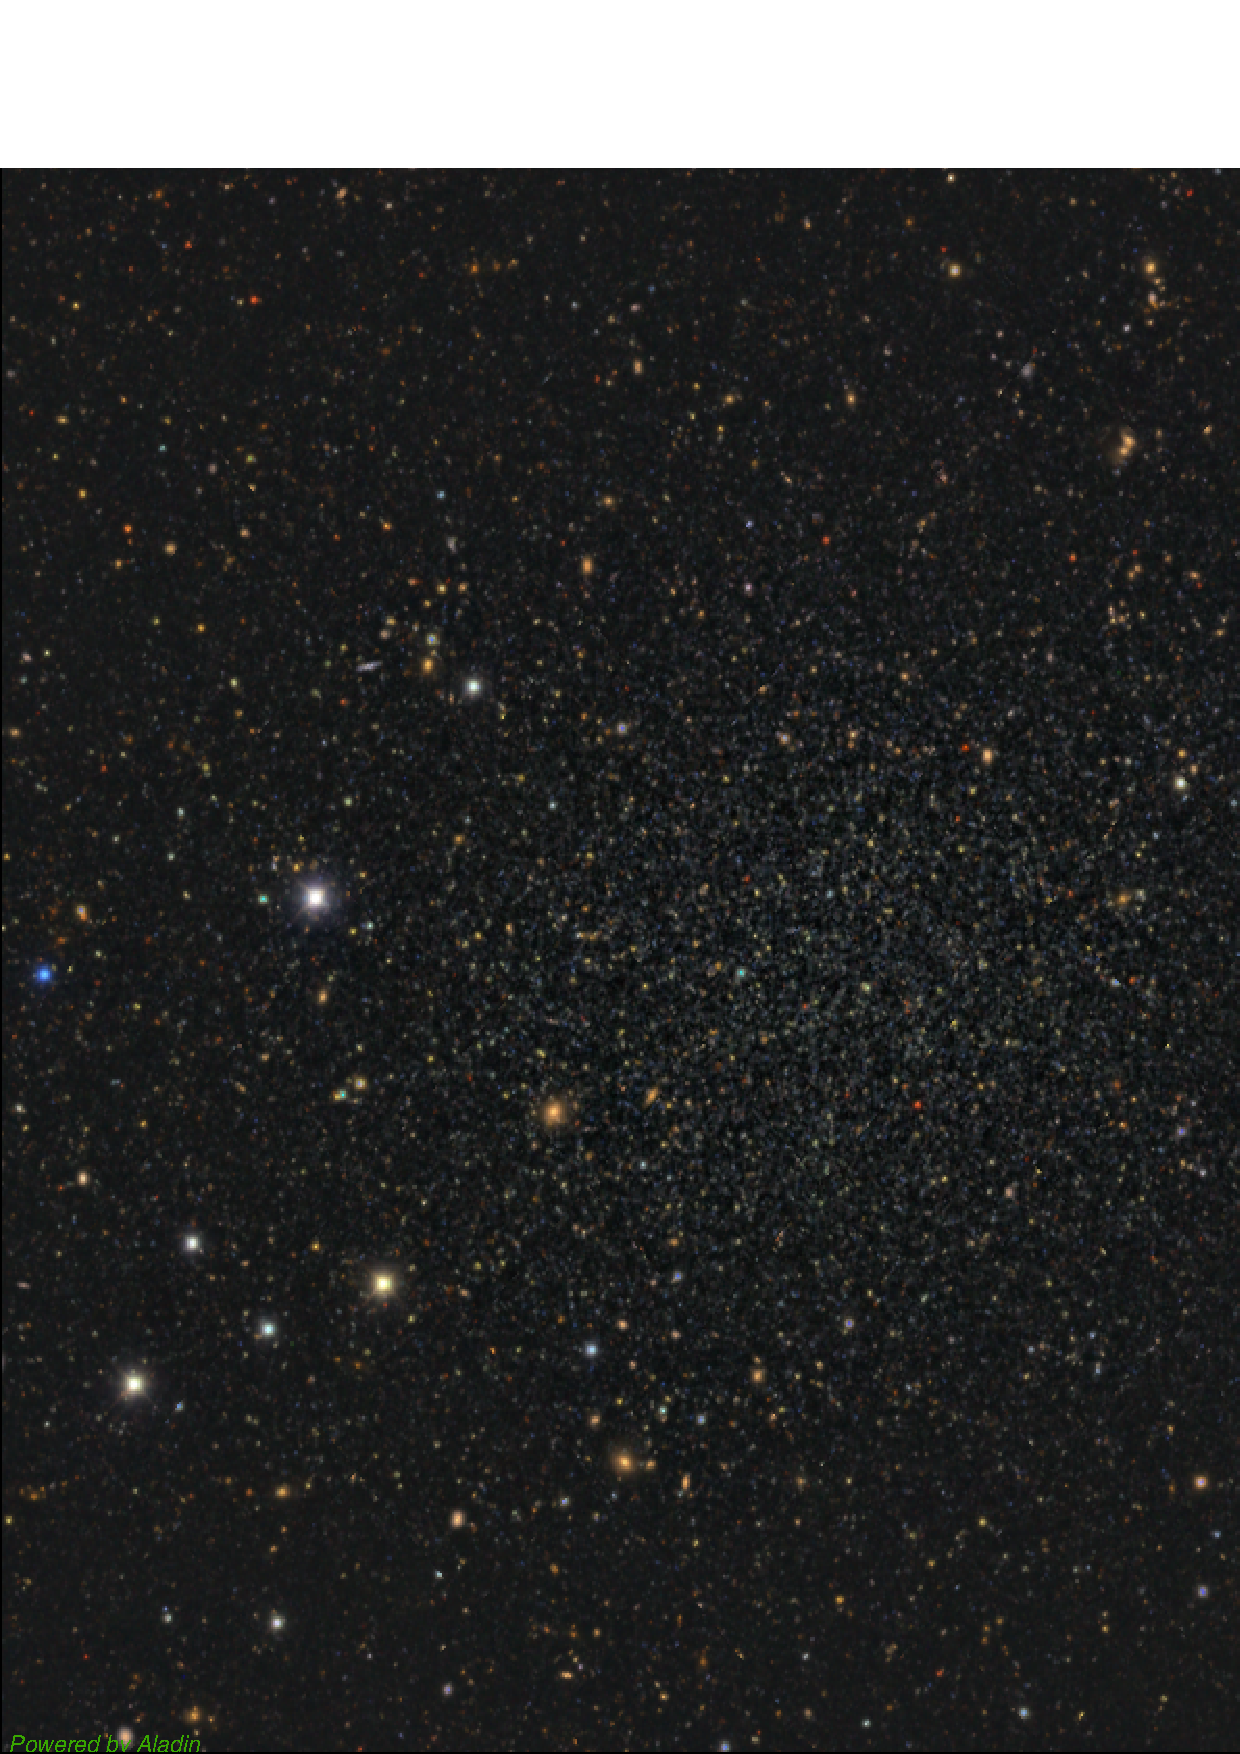
\includegraphics[width=5.41667in,height=5.41667in]{figures/scl_des_dr2.png}
\caption[scl\_image]{Sculptor image from DES DR 2 via
HiPS2FITS.}\label{fig:scl_image}
\end{figure}

\begin{figure}
\centering
\includegraphics{figures/scl_umi_vs_penarrubia.pdf}
\caption[Idealized simulations match Scl and UMi]{Sculptor and UMi's
profiles are well-matched to \citet{PNM2008}.}\label{fig:toy_profiles}
\end{figure}

\section{}\label{section}

Sculptor (Scl) is one of the first discovered dwarf galaxies of the
Milky Way (Shapley 1938; only preceded by the SMC and LMC!). As a
classical dwarf spheroidal, Scl is relatively bright and compact.

Since the initial discovery of Scl, most authors have noted that Scl has
a slight ellipticity (\(0.36\)), often attributed to tidal effects.
However, this does not align with the absolute proper motion or orbital
path of the galaxy.

While Scl has a relatively large pericentre (greater than 50kpc),
\citet{Sestito+23} detect that the galaxy likely has an excess of stars
in the outskirts (past about 60 arcminutes). This excess is perhaps one
of the clearest indications that Scl may be affected by tides. Here, our
goal is to determine if under a \(\Lambda\) CMD paradigm with DM-only
simulations, tidal effects of the Milky Way (or LMC) may indeed be
consistent with these observations, or if these observations may reveal
instead a extended stellar ``halo'' or second component of the
galaxy---illustrating a complex formation for the galaxy.

Figure: Image of Sculptor from DES.

Theoretical work on Sculptor

\begin{itemize}
\tightlist
\item
  \citet{battaglia+2008}
\item
  \citet{iorio+2019}
\end{itemize}

Observational work on Scl

\begin{itemize}
\tightlist
\item
  \citet{sestito+2023a}
\item
  \citet{tolstoy+2023}, \citet{arroyo-polonio+2023},
  \citet{arroyo-polonio+2024}
\item
  \citet{eskridge1988}
\end{itemize}

\begin{table*}[t]
\centering
\caption{Measured properties of Sculptor}
\label{tbl:Measured-properties-of-Sculptor}
\begin{tabular}{lll}
\toprule
parameter & value & Source\\
\midrule
$\alpha$ & $15.0183 \pm 0.0012$˚ & M+18\\
$\delta$ & $-33.7186 \pm 0.00072$˚ & M+18\\
distance & $83.2 \pm 2$ kpc & Tran+22\\
$\mu_\alpha \cos \delta$ & $0.099 \pm 0.002 \pm 0.017$ mas yr$^{-1}$ & MV20a\\
$\mu_\delta$ & $-0.160 \pm 0.002_{\rm stat} \pm 0.017_{\rm sys}$ mas yr$^{-1}$ & MV20a\\
RV & $111.4 \pm 0.2$ & This work\\
$\sigma_v$ & $9.61\pm0.16$ & This work\\
$R_h$ & $12.33 \pm 0.05$ arcmin & MV20*\\
$R_h$ & $8.69 \pm 0.2$ arcmin & this work?\\
ell & $0.36 \pm 0.01$ & M+18\\
PA & $92\pm1$ & M+18\\
$M_V$ & $-10.82\pm0.14$ & M+18\\
\bottomrule
\end{tabular}
\end{table*}

Can I just cite \citet{arroyo-polonio+2024} for velocity information for
Sculptor? They correct for binary and do a more detailed discussion of
rotation.

\subsection{Ursa Minor}\label{ursa-minor}

\begin{itemize}
\item
  \citet{sestito+2023b}
\item
  \citet{pace+2020}
\end{itemize}

\begin{figure}
\centering
\includegraphics[width=5.41667in,height=5.41667in]{figures/umi_image.jpg}
\caption[Ursa Minor Image]{Ursa Minor Dwarf. Composite Public
data/Giuseppe Donatiello. Updated image in 2022.
https://www.flickr.com/photos/133259498@N05/page8}\label{fig:umi_image}
\end{figure}

\begin{table*}[t]
\centering
\caption{Measured properties of Ursa Minor}
\label{tbl:Measured-properties-of-Ursa-Minor}
\begin{tabular}{lll}
\toprule
parameter & value & Source\\
\midrule
$\alpha$ & $ 227.2420 \pm 0.0045$˚ & M+18\\
$\delta$ & $67.2221 \pm 0.00158$˚ & M+18\\
distance & $70.1 \pm 2.9$ kpc & \\
$\mu_\alpha \cos \delta$ & $-0.124 \pm 0.004 \pm 0.017$ mas yr$^{-1}$ & MV20a\\
$\mu_\delta$ & $0.078 \pm 0.004_{\rm stat} \pm 0.017_{\rm sys}$ mas yr$^{-1}$ & MV20a\\
RV & $-245 \pm 1$ km s$^{-1}$ & This work\\
$\sigma_v$ & $9 \pm 0.6$ & This work\\
$r_h$ & $18.2 \pm 0.1$ arcmin & M+18\\
ell & $0.55 \pm 0.01$ & M+18\\
PA & $50 \pm 1^\circ$ & M+18\\
$M_V$ & $-9.03 \pm 0.05$ & M+18\\
\bottomrule
\end{tabular}
\end{table*}

\subsection{Theoretical Background}\label{theoretical-background}

\begin{itemize}
\tightlist
\item
  Cosmology foundations
\item
  NFW plot (density or energy), maybe borrow from paper?

  \begin{itemize}
  \tightlist
  \item
    Explain origin of NFW
  \end{itemize}
\item
  Dwarf galaxy formation, halos
\item
  Evolution under tidal field
\item
\end{itemize}

To motivate why a tidal interaction may give rise to the observed
density profiles, we create a toy simulation following \citet{PNM2008}.

\begin{itemize}
\item
  NFW initial conditions (sculptor like, vcm, rcm)
\item
  Evolved in x-y plane using \citet{EP2020} potential for
  \textasciitilde{} 5Gyr with pericentre of 15 kpc and apocentre of 100
  kpc.
\item
  Exponential initial stellar profile.
\end{itemize}

As a dark matter halo is perturbed on a pericentric passage with the
milky way,

\begin{itemize}
\tightlist
\item
  Tidal stress heats halo slightly
\item
  Mass loss, particularly of loosely bound particles
\end{itemize}

The stellar component tracers will similarly follow the behaviour of the
dark matter.

An emperical estimate of where the simulation's stars are becoming
unbound is, as stated in \citet{PNM2008}, the break radius \[
R_b = C\,\sigma_{v}\,\Delta t
\] where \(\sigma_v\) is the present line of sight velocity dispersion ,
\(\delta t\) is the time since pericentre, and \(C \approx 0.55\) is a
fit. The idea motivating this equation is stars in the inner regions
will have dynamically equilibriated to the new potential (phase mixed),
however the outer regions are no longer in steady state, so we have to
wait until the crossing time reaches them as well.

As illustrated in fig.~\ref{fig:toy_profiles}, the density profile
initially stars off exponential. At increasing times since the first
pericentric passage, the break radius, appearing as an apparent
separation between the slopes of the inner and outer profile, increases.
